\documentclass[11pt]{article}

\usepackage{amsmath}
\usepackage{amssymb}
\usepackage{amsthm}
\usepackage{mathtools}
\usepackage{xcolor}
\usepackage{algorithm}
\usepackage{algorithmic}

\newtheorem{theorem}{Theorem}
%! TEX root = main.tex
\usepackage{xcolor}
\usepackage{algorithm}
\usepackage{algpseudocode}
\usepackage{hyperref}

%\newcommand{\deltat}{\delta\hspace*{-.3mm}t}
\newcommand{\deltat}{\ensuremath{\delta\hspace{-.06em}t}}
\newcommand{\bigO}[1]{O (#1)}
\newcommand{\reward}{\tilde{r}}
\newcommand{\actionspace}{\mathcal{A}}
\newcommand{\statespace}{\mathcal{S}}
\newcommand{\NDC}[1]{\color{red}NDC:#1\color{black}}

\newcommand{\pfield}{\mathcal{F}_t}
\newcommand{\Ep}[1]{\BE\left[#1\mid\pfield\right]}
\newcommand{\diag}[1]{\mathrm{\textbf{diag}}(#1)}
\newcommand{\lmax}{\lambda_{\mathrm{max}}}



\newcommand{\mynumero}{n°}


%\def\d{{\mathrm{d}}}
%\def\d{\operatorname{d}\!}
\def\d{\operatorname{d}\!{}}
%\def\d{\operatorname{}\!\mathrm{d}}

\def\N{{\mathbb{N}}}
\def\Z{{\mathbb{Z}}}
\def\Nstar{{\mathbb{N}^\star}}
\def\Q{{\mathbb{Q}}}
\def\R{{\mathbb{R}}}
\def\C{{\mathbb{C}}}

\renewcommand{\geq}{\geqslant}
\renewcommand{\leq}{\leqslant}

\renewcommand{\emptyset}{\varnothing}

\newcommand{\deq}{\mathrel{\mathop{:}}=}
\newcommand{\eqd}{=\mathrel{\mathop{:}}}

\newcommand{\from}{\colon} % correct ':' in f\from X \to Y
\newcommand{\st}{\mid} % set builder
%\newcommand{\st}{\mathrel{}\middle|\mathrel{}} % set builder

\def\eps{\varepsilon}
\renewcommand{\epsilon}{\varepsilon}
\renewcommand{\phi}{\varphi}

\def\ds{\displaystyle}

\DeclareMathOperator{\dist}{dist}
\DeclareMathOperator{\diam}{diam}
\DeclareMathOperator{\vol}{vol}
\DeclareMathOperator{\Ric}{Ric}

\DeclareMathOperator{\lap}{\Delta\!}
\DeclareMathOperator{\nab}{\nabla\!\!}
\DeclareMathOperator{\Hess}{Hess}

\DeclareMathOperator{\Ent}{Ent}
\DeclareMathOperator{\Var}{Var}
\DeclareMathOperator{\Cov}{Cov}
\let\oldPr\Pr
\renewcommand{\Pr}{\oldPr\nolimits}
\newcommand{\E}{\mathbb{E}}
\newcommand{\KL}[2]{\mathrm{KL}\!\left(#1 \,|\hspace{-.15ex}|\,#2\right)}

\DeclareMathOperator{\mult}{mult}
\DeclareMathOperator{\Card}{Card}
\DeclareMathOperator{\Aut}{Aut}
\DeclareMathOperator{\Epi}{Epi}
\DeclareMathOperator{\Spec}{Sp}
%\DeclareMathOperator{\Ker}{Ker}
\DeclareMathOperator{\Img}{Im}
\DeclareMathOperator{\Tr}{Tr}
\DeclareMathOperator{\tr}{tr}
\DeclareMathOperator{\Tor}{Tor}
\DeclareMathOperator{\Ext}{Ext}
\DeclareMathOperator{\Hom}{Hom}
\DeclareMathOperator{\End}{End}
\DeclareMathOperator{\coker}{coker}
\DeclareMathOperator{\Id}{Id}
\DeclareMathOperator{\id}{id}
%\DeclareMathOperator{\diag}{diag}


\newcommand{\abs}[1]{\left\lvert#1\right\rvert}
\newcommand{\norm}[1]{\left\lVert#1\right\rVert}
\newcommand{\scal}[2]{\left< \, #1 \mid #2 \, \right>}
\newcommand{\1}{\mathbbm{1}}

\newcommand{\ilim}[1]{\underset{#1}{\underrightarrow{\lim\vspace{.5ex}}}\,}
\newcommand{\plim}[1]{\underset{#1}{\underleftarrow{\lim\vspace{.5ex}}}\,}

\DeclareMathOperator*{\vlimsup}{\varlimsup}
\DeclareMathOperator*{\vliminf}{\varliminf}

\newcommand{\presgroup}[2]{\left\langle\,#1 \mid  #2\,\right\rangle}

\newcommand{\twopi}{2\hspace{-.23em}\pi}

%\DeclareMathOperator*{\argmax}{arg\,max}
%\DeclareMathOperator*{\argmin}{arg\,min}



\begin{document}
\section{Proofs}

We now give proofs for all the results presented in the paper. Most
proofs follow standard patterns from calculus and numerical schemes for
differential equations, except for Theorem~\ref{thm:policyimprovement},
which uses an argument specific to reinforcement learning to prove that
the continuous-time advantage function contains all the necessary
information for policy values.


The first result presented is a proof of convergence for discretized
trajectories.
\begin{theorem}
	Let $F\from {\cal S} \times {\cal A} \rightarrow \bb{R}^n$ and $\pi\from {\cal S}
	\rightarrow {\cal A}$ be the dynamic and policy functions. Assume that,
	for any $a$, $s \rightarrow F(s, a)$ and $s \rightarrow F(s, \pi(s))$
	are ${\cal C}^1$, bounded and $K$-lipschitz.  For
	a given $s_0$, define the trajectory $(s_t)_{t\geq 0}$ as the unique
	solution of the differential equation
	\begin{equation}
		\frac{ds_t}{dt} = F(s_t, \pi(s_t)).
		\label{eq:diff}
	\end{equation}
	For any $\deltat > 0$, define the discretized trajectory
	$(s_\deltat^k)_k$ which amounts to maintaining each action for a
	time interval $\deltat$; it is defined by induction as $s_\deltat^0 = s_0$,
	$s_\deltat^{k + 1}$ is the value at time $\deltat$ of
	the unique solution of
	\begin{equation}
		\frac{d\tilde{s}_t}{dt} = F(\tilde{s}_t, \pi(s_\deltat^k))
		\label{eq:diff_2}
	\end{equation}
	with initial point $s_\deltat^k$.
	Then, there exists $C > 0$ such that, for every $t \geq 0$
	\begin{equation}
		\|s_t - s_\deltat^{\lfloor \frac{t}{\deltat} \rfloor}\|
		\leq \deltat \frac{C}{K}e^{Kt}.
	\end{equation}
	Therefore, discretized trajectories converge pointwise to continuous trajectories.
	\label{th:traj-conv}
\end{theorem}
\begin{proof}
	%! TEX root = icml_drau.tex

\end{proof}

In what follows, we assume that the continuous-time reward function $r\from {\cal S} \times {\cal A} \rightarrow \bb{R}$
is bounded, to ensure existence of $V^\pi$ and $V^\pi_\deltat$ for all $\deltat$
.\begin{theorem}
	Assume that $r\from {\cal S} \times {\cal A} \rightarrow \bb R$ is bounded, and
	that $s \rightarrow r(s, \pi(s))$ is $L_r$-Lipschitz continuous, then
	for all $s \in {\cal S}$, one has
	%\begin{equation}
	%\label{eq:conv-value}
	$V^\pi_\deltat(s) = V^\pi(s) + \smallo(\deltat)$
	%\end{equation}
	Lhen $\deltat\to 0$.
	\label{th:conv-value}
\end{theorem}
\begin{proof}
	%! TEX root = icml_drau.tex


\end{proof}

For the following proof, we further assume that both $V^\pi$ and
$V^\pi_\deltat$ are continuously differentiable, and that the gradient and
Hessian of $V^\pi_\deltat$ w.r.t. $s$ are uniformly bounded in both $s$ and $\deltat$.
We also assume convergence of $\partial_s V^\pi_\deltat(s)$ to $\partial_s V^\pi(s)$ for
all $s$.

\begin{theorem}
	Under the hypothesis above, there exists $A^\pi\from {\cal S} \rightarrow
	\bb{R}$ such that $A^\pi_\deltat$ converges pointwise to $A^\pi$ as
	$\deltat$ goes to $0$. Besides,
	\begin{equation}
		A^\pi(s, a) = r(s, a) + \partial_s V^\pi(s) F(s, a) + \log \gamma V^\pi(s).
	\end{equation}\end{theorem}
\begin{proof}
	%! TEX root = icml_drau.tex


\end{proof}

We now show that policy improvement works with the continous time advantage function, i.e.\
\begin{theorem}
\label{thm:policyimprovement}
	Let $\pi$ and $\pi'$ be two policies such that both $s \rightarrow r(s, \pi(s))$ and
	$s \rightarrow r(s, \pi'(s))$ are continuous.
	Assume that both $V^\pi$ and $V^{\pi'}$ are continuously differentiable.
	Define the advantage function for policies $\pi$ and $\pi'$ as in Eq.~\eqref{eq:adv_function}.

	If for all $s$, $A^\pi(s, \pi'(s)) \geq 0$, then for all $s$,
	$V^\pi(s) \leq V^{\pi'}(s)$. Moreover, if for all $s$, 
	$V^{\pi'}(s)>V^{\pi}(s)$, then there exists $s'$ such that $A^\pi(s',\pi'(s'))>0$.
\end{theorem}

\begin{proof}
	%! TEX root = supplementary.tex
Let $(s_t)_{t\geq 0}$ be a trajectory sampled from $\pi'$ i.e.\ solution of the equation
\begin{equation}
	ds_t / dt = F(s_t, \pi'(s_t))
\end{equation}
with initial condition $s_0 = s$.

Define
\begin{equation}
	B(T) = \int_{t=0}^T \gamma^t r(s_t, \pi'(s_t)) dt + \gamma^T V^\pi(s_T).
\end{equation}
This function if continuously differentiable, and its derivative is
\begin{align}
	\dot{B}(T) &= \gamma^T r(s_T, \pi'(s_T)) + \gamma^T \partial_s V^\pi(s) F(s, \pi'(s)) + \gamma^T \ln(\gamma) V^\pi(s_T)\\
		   &= \gamma^T A^\pi(s_T, \pi'(s))
		   &\geq 0.
\end{align}
Thus $B$ is increasing, and $B(0) = V^\pi(s)$, $\lim\limits_{T\rightarrow \infty} B(t) = V^{\pi'}(s)$.
Consequently, $V^\pi(s) \leq V^{\pi'}(s)$, which ends the proof.


\end{proof}
\begin{theorem}
	Let $\cal A = \bb R^A$ be the action space, and let ${\cal P}_1 = \bb
	R^{p_1}$ and ${\cal P}_2 = \bb R^{p_2}$ be parameter spaces.  Let
	$A\colon {\cal P}_1 \times {\cal S} \times {\cal A} \rightarrow \bb R$
	and $V\colon {\cal P}_2 \times {\cal S} \rightarrow \bb R$ be ${\cal
	C}^2$ function approximators with bounded gradients and Hessians. Let
	$(a_t)_{t\geq 0}$ be a ${\cal C}^1$ exploratory actions trajectory and
	$(s_t)_{t\geq 0}$ the resulting state trajectory, when starting from $s_0$ and
	verifying Eq.~\eqref{eq:diff}.  Let $\theta^k_\deltat$ and
	$\psi^k_\deltat$ be the discrete parameter trajectories resulting from
	the gradient descent steps in the main text, with
	learning rates $\eta^V = \alpha^V \deltat^\beta$ and $\eta^A = \alpha^A \deltat^\beta$. Then,
	\begin{itemize}
		\item If $\beta = 1$ the discrete parameter trajectories converge to continuous parameter
			trajectories as $\deltat$ goes to $0$.
		\item If $\beta > 1$, parameter trajectories become
		stationary as
			$\deltat$ goes to $0$.
		\item If $\beta < 1$, parameters can grow arbitrarily large after an arbitrarily small physical time when $\deltat$ goes to $0$.
	\end{itemize}
\end{theorem}
\begin{proof}
	%! TEX root = icml_drau.tex


	%! TEX root = supplementary.tex
We now turn to proving that when $\beta < 1$,
trajectories can diverge instantly in physical time. 
Consider the following actionless continuous MDP, 
\begin{equation}
	s_t = \sin(t)
\end{equation}
with reward $0$ everywhere and $0 < \gamma < 1$.
The resulting value function is $V(s) = 0$ (since there
are no actions, $V$ is independent of a policy).
We consider the function approximator $V_\theta(s) = \theta s$.
The update rule for $\theta$ is
\begin{align}
	\theta_\deltat^{k+1} &= \theta_\deltat^k + \alpha \deltat^\beta \frac{\gamma^\deltat \theta_\deltat^k \sin((k + 1) \deltat) - \theta_\deltat^k \sin(k\deltat)}{\deltat}\\
			     &= \theta_\deltat^k + \alpha \deltat^\beta (\ln \gamma \theta_\deltat^k \sin(k \deltat) + \theta_\deltat^k \cos(k \deltat)) + \bigO(\deltat^{\beta + 1})\\
			     &= \theta_\deltat^k(1 + \alpha \deltat^\beta (\ln \gamma \sin(k \deltat) + \cos(k \deltat))) + \bigO(\deltat^{\beta + 1}).
\end{align}
Let $\rho_\deltat^k = \log \theta_\deltat^k$,
\begin{align}
	\rho_\deltat^k = \rho_\deltat^k + \alpha \deltat^\beta (\ln \gamma \sin(k \deltat) + \cos(k \deltat)) + \bigO(\deltat^{2\beta}).
\end{align}
Then, let $K_\deltat = \lfloor \deltat^{-\frac{\beta + 3}{4}}\rfloor$,
\begin{align}
	\rho_\deltat^{K_\deltat} &= \rho_\deltat^0 + \alpha \deltat^\beta \sum\limits_{k=0}^{K_\deltat} (\ln \gamma k\deltat + 1)k\deltat + \bigO(K_\deltat K_\deltat^3 \deltat^{3 + \beta}) + \bigO(\deltat^{2\beta})\\
				 &= \rho_\deltat^0 + \alpha \deltat^\beta \sum\limits_{k=0}^{K_\deltat} (\ln \gamma k\deltat + 1)k\deltat + \bigO(1)\\
				 &= \rho_\delta^0 + \alpha\deltat^{\beta + 2} \ln\gamma \frac{K_\deltat (K_\deltat + 1) (2 K_\deltat + 1)}{6} + \alpha \deltat^{\beta + 1} \frac{K_\deltat (K_\deltat + 1)}{2} + \bigO(\deltat^{2 - 2 \beta})\\
				 &= \alpha \frac{\deltat^{\frac{\beta - 1}{2}}}{2} + \smallo(\deltat^{\frac{\beta - 1}{2}})\\
				 &\xrightarrow[\deltat\to 0]{} +\infty.
\end{align}
Thus parameters diverge in an infinitesimal physical time when $\deltat$ goes to $0$.


\end{proof}

      \begin{theorem}
	Exploration strategy
\end{theorem}
\begin{proof}
	%! TEX root = icml_drau.tex
% Let $\deltat_1 > 0$. 

\begin{align}
  s_{t + \deltat} &= s_t + \sum_{k=1}^{\lfloor 1/\deltat\rfloor} s_{t+k\deltat^2} -  s_{t+(k-1)\deltat^2} + \bigO(\deltat^2) \\
                    &= s_t + \sum_{k=1}^{\lfloor 1/\deltat \rfloor} F(s_{t+(k-1)\deltat^2}, a_k)\deltat^2 + \bigO(\deltat^2)
                    % &= s_t + \sum_{k=1}^{\lfloor \deltat_1/\deltat\rfloor} \left(F(s_{t}, a_k) + \bigO(k\deltat)\right)\deltat + \bigO(\deltat) \\
                    % &= s_t + \sum_{k=1}^{\lfloor \deltat_1/\deltat\rfloor} F(s_{t}, a_k) \deltat + \bigO(\deltat_1^2) + \bigO(\deltat) 
\end{align}

If we define $f(s) \deq \E_{a \sim \pi(s)}\left[F(s, a)\right]$, then $f$ is \TODO{smooth enough}. We have: 

  \begin{align}
    s_{t + \deltat}   & = s_t + \sum_{k=1}^{\lfloor 1/\deltat\rfloor} f(s_{t+(k-1)\deltat})\deltat^2 + \sum_{k=1}^{\lfloor 1/\deltat\rfloor} (F(s_{t+(k-1)\deltat^2}, a_k) - f(s_{t+(k-1)\deltat^2}))\deltat^2 + \bigO(\deltat^2)        \\
  \end{align}

  We define $\xi \deq \sum_{k=1}^{\lfloor 1/\deltat\rfloor} (F(s_{t+(k-1)\deltat^2}, a_k) - f(s_{t+(k-1)\deltat^2}))\deltat^2$. We have:
  \begin{align}
    \E[\xi] &= 0 \\
    \E[\|\xi\|^2] &= \bigO(\deltat^3)
  \end{align}

  Therefore:
  \begin{align}
  s_{t + \deltat}  &= s_t + \sum_{k=1}^{\lfloor 1/\deltat\rfloor} \left(f(s_{t}) + \bigO(k\deltat^2)\right)\deltat^2 + \xi + \bigO(\deltat^2) \\
                      & = s_t + f(s_{t}) \deltat + \xi + \bigO(\deltat^2) 
  \end{align}

  Therefore, we have $a>0$ such that $\|s_{t + \deltat} - s_t - f(s_t)\deltat\| \leq \|\xi\| + a\deltat^2$
  
We define $\tilde s_\deltat^{k+1} \deq f(s_\deltat^k)\deltat$. We have:

\begin{align}
  \|s_{t+(k+1)\deltat} - \tilde{s}_\deltat^{k+1}\| &\leq
                                                     \|s_{t+(k+1)\deltat} - s_t - f(s_t)\deltat\| + \|s_t + f(s_t)\deltat - \tilde{s}_\deltat^{k+1}\|\\
  &\leq \|\xi_k\| + a\deltat^2 + (1+L_f\deltat)\|s_{t+k\deltat} - \tilde{s}_\deltat^{k}\|
\end{align}
where $L_f$ is the Lipschitz constant of $f$ \TODO{justify}.
%We define $w_k = \|s_{t+k\deltat} - \tilde{s}_\deltat^{k}\|$. We have:
By induction, we have:
\begin{align}
  w_{k+1} \leq \|\xi_k\| + a\deltat^2 + (1+L_f\deltat)\|s_{t+k\deltat} - \tilde{s}_\deltat^{k}\|w_k
\end{align}
By induction:
\begin{align}
  \|s_{t} - \tilde{s}_\deltat^{\lfloor t/\deltat \rfloor} \| \leq \frac{a\deltat}{L_f}\exp(L_ft) + \sum_{j=0}^{\lfloor t/\deltat \rfloor}(1+\deltat L_f)^j\|\xi_j\|  
\end{align}

Therefore, if $\varepsilon >0$, we have:
\begin{align}
  \BP\left(\|s_{t} - \tilde{s}_\deltat^{\lfloor t/\deltat \rfloor} \| > \varepsilon \right) &\leq \BP\left(\sum_{j=0}^{\lfloor t/\deltat \rfloor}(1+\deltat L_f)^j\|\xi_j\| > \varepsilon - \frac{a\deltat}{L_f}\exp(L_ft)\right) \\
                                                                                            &\leq \frac{\E\left[\sum_{j=0}^{\lfloor t/\deltat \rfloor}(1+\deltat L_f)^j\|\xi_j\|\right]}{\varepsilon - \frac{a\deltat}{L_f}\exp(L_ft)}\\
                                                                                            &\leq \frac{\E\left[\|\xi\|\right]}{\varepsilon - \frac{a\deltat}{L_f}\exp(L_ft)}\frac{\exp(L_ft)}{L_f\deltat}\\
  % &\leq \frac{\sqrt{\E\left[\|\xi\|^2\right]}}{\varepsilon - \frac{a\deltat}{L_f}\exp(L_ft)}\frac{\exp(L_f\deltat)}{L_f\deltat}\\
\end{align}
But $\E\left[\|\xi\|\right] \leq \sqrt{\E\left[\|\xi\|^2\right]} \leq \sigma \deltat^{3/2}$. Therefore, we have:
\begin{align}
  \BP\left(\|s_{t} - \tilde{s}_\deltat^{\lfloor t/\deltat \rfloor} \| > \varepsilon \right) & = \bigO(\sqrt \deltat)
\end{align}

Therefore, the random process $s_t$ converge in probability to $\tilde s$. Furthermore, by a similar argument than in Theorem \TODO{the first one}, we know that the discretized process $\tilde s$ converge to the continuous process defined by $\frac{ds}{dt} = f(s_t)$. We can conclude ou result.

% We define for all $0 \leq j \leq \lfloor t/\deltat \rfloor$: $\alpha_j = \omega (1+\deltat L_f)^j$, such that $\sum_j \alpha_j = 1$. Then, we have:
% \begin{align}
%   \BP\left( \sum_{j=0}^{\lfloor t/\deltat \rfloor}(1+\deltat L_f)^j\|\xi_j\| > \varepsilon'\right) & \leq \BP\left( \exists j,  (1+\deltat L_f)^j\|\xi_j\| > \alpha_j\varepsilon'\right) \\
%                                                                                                    & \leq \sum_j \BP\left(  (1+\deltat L_f)^j\|\xi_j\| > \alpha_j\varepsilon'\right)     \\
%                                                                                                    & \leq \sum_j \BP\left(\|\xi_j\| > \omega \varepsilon'\right) \\
%   &\leq \frac{t\sigma^2\deltat^2}{\omega^2 \varepsilon'^2}
% \end{align}
% Moreover, we have $\omega \leq \frac{\exp(L_f t)}{L_f \deltat}$. We have:
% \begin{align}
%   \BP\left( \sum_{j=0}^{\lfloor t/\deltat \rfloor}(1+\deltat L_f)^j\|\xi_j\| > \varepsilon'\right) &\leq  t\sigma\deltat\frac{\exp(L_f t)}{L_f}
% \end{align}
% Finally:
% \begin{align}
%   \BP\left(\|s_{t} - \tilde{s}_\deltat^{\lfloor t/\deltat \rfloor} \| > \varepsilon \right) \leq \BP\left(\sum_{j=0}^{\lfloor t/\deltat \rfloor}(1+\deltat L_f)^j\|\xi_j\| > \varepsilon - \frac{a\deltat}{L_f}\exp(L_ft)\right)
% \end{align}
%%% Local Variables:
%%% TeX-master: "icml_drau"
%%% End:


\end{proof}
\section{Implementation details}
%! TEX root = supplementary.tex
All the details specifying our implementation are given in this section. We
first give precise pseudo code descriptions for both \emph{Continuous Deep
Advantage Updating} (Alg.~\ref{alg:cdau}), as well as the variants of DDPG
(Alg.~\ref{alg:ddpg}) and DQN (Alg.~\ref{alg:dqn}) used.

\begin{algorithm}
	%! TEX root = supplementary.tex

\begin{algorithmic}
	\STATE \textbf{Inputs:}
	\STATE $\theta$, $\psi$ and $\phi$, parameters of
	$V_{\theta}$, $\bar{A}_{\psi}$ and $\pi_\phi$.
	\STATE $\pi^{\text{explore}}$ and $\nu_\deltat$ defining an exploration policy.
	\STATE \textbf{opt}$_V$, \textbf{opt}$_A$, \textbf{opt}$_\pi$, $\alpha^V \deltat$, $\alpha^A \deltat$ and $\alpha^\pi\deltat$, optimizers and learning rates.
	\STATE $\mathcal{D}$, buffer of transitions $(s, a, r, d, s')$, with $d$ the episode termination signal.
	\STATE $\deltat$ and $\gamma$, time discretization and discount factor.
	\STATE \textbf{nb\_epochs} number of epochs.
	\STATE \textbf{nb\_steps}, number of steps per epoch.
	\STATE
	\STATE Observe initial state $s^0$
	\STATE $t \gets 0$
	\FOR {$e=0, \textbf{nb\_epochs}$}
	\FOR {$j=1, \textbf{nb\_steps}$}
	\STATE $a^k \leftarrow \pi^{\text{explore}}(s^k, \nu^k_\deltat)$.
	\STATE Perform $a^k$ and observe $(r^{k+1}, d^{k+1}, s^{k+1})$.
	\STATE Store $(s^k, a^k, r^{k+1}, d^{k+1}, s^{k+1})$ in $\mathcal{D}$.
	\STATE $k \gets k + 1$
	\ENDFOR
	\FOR {$k=0, \text{nb\_learn}$}
	\STATE \text{Sample a batch of $N$ random transitions from $\mathcal{D}$}
	\STATE $Q^i \gets V_{\theta}(s^i) + \deltat\hspace{-.17em}\left(
	\bar{A}_{\psi}(s^i, a^i) - \bar{A}_{\psi}(s^i, \pi_\phi(s^i))\right)$
	\STATE $\tilde{Q^i} \gets r^i\deltat + (1 - d^i) \gamma^{\deltat} V_{\theta}(s'^i)$
	\STATE $\Delta \theta \gets \frac{1}{N}\sum\limits_{i=1}^N  \frac{\left(Q^i - \tilde{Q^i}\right)\partial_{\theta} V_{\theta}(s^i)}{\deltat}$
	\STATE $\Delta \psi \gets \frac{1}{N}\sum\limits_{i=1}^N \frac{\left(Q^i - \tilde{Q^i}\right)\partial_{\psi} \left(\bar{A}_{\psi}(s^i, a^i) - \bar{A}_{\psi}(s^i, \pi_\phi(s^i))\right) }{\deltat}$
	\STATE $\Delta \phi \gets \frac{1}{N} \sum\limits_{i=1}^N \partial_a \bar{A}_\psi(s^i, \pi_\phi(s^i)) \partial_\phi \pi_\phi(s^i)$
	\STATE Update $\theta$ with \textbf{opt}$_V$, $\Delta \theta$ and learning rate $\alpha^V \deltat$.
	\STATE Update $\psi$ with \textbf{opt}$_A$, $\Delta \psi$ and learning rate $\alpha^A \deltat$.
	\STATE Update $\phi$ with \textbf{opt}$_\pi$, $\Delta \phi$ and learning rate $\alpha^\pi \deltat$.
	\ENDFOR
	\ENDFOR
\end{algorithmic}

	\caption{Continuous DAU}
	\label{alg:cdau}
\end{algorithm}
\begin{algorithm}
	%! TEX root = supplementary.tex

\begin{algorithmic}
	\STATE \textbf{Inputs:}
	\STATE $\psi$ and $\phi$, parameters of
	$Q_\psi$ and $\pi_\phi$.
	\STATE $\psi'$ and $\phi'$, parameters of target networks
	$Q_{\psi'}$ and $\pi_{\phi'}$.
	\STATE $\pi^{\text{explore}}$ and $\nu$ defining an exploration policy.
	\STATE \textbf{opt}$_Q$, \textbf{opt}$_\pi$, $\alpha^Q$ and $\alpha^\pi$, optimizers and learning rates.
	\STATE $\mathcal{D}$, buffer of transitions $(s, a, r, d, s')$, with $d$ the episode termination signal.
	\STATE $\gamma$ discount factor.
	\STATE $\tau$ target network update factor.
	\STATE \textbf{nb\_epochs} number of epochs.
	\STATE \textbf{nb\_steps}, number of steps per epoch.
	\STATE
	\STATE Observe initial state $s^0$
	\STATE $t \gets 0$
	\FOR {$e=0, \textbf{nb\_epochs}$}
	\FOR {$j=1, \textbf{nb\_steps}$}
	\STATE $a^k \leftarrow \pi^{\text{explore}}(s^k, \nu^k)$.
	\STATE Perform $a^k$ and observe $(r^{k+1}, d^{k+1}, s^{k+1})$.
	\STATE Store $(s^k, a^k, r^{k+1}, d^{k+1}, s^{k+1})$ in $\mathcal{D}$.
	\STATE $k \gets k + 1$
	\ENDFOR
	\FOR {$k=0, \text{nb\_learn}$}
	\STATE \text{Sample a batch of $N$ random transitions from $\mathcal{D}$}
	\STATE $\tilde{Q^i} \gets r^i + (1 - d^i) \gamma Q_{\psi'}(s'^i, \pi_{\phi'}(s'^i))$
	\STATE $\Delta \psi \gets \frac{1}{N}\sum\limits_{i=1}^N \left(Q^i - \tilde{Q^i}\right) \partial_\psi Q(s^i, a^i)$
	\STATE $\Delta \phi \gets \frac{1}{N} \sum\limits_{i=1}^N \partial_a Q_\psi(s^i, \pi_\phi(s^i)) \partial_\phi \pi_\phi(s^i)$
	\STATE Update $\psi$ with \textbf{opt}$_Q$, $\Delta \psi$ and learning rate $\alpha^Q$.
	\STATE Update $\phi$ with \textbf{opt}$_\pi$, $\Delta \phi$ and learning rate $\alpha^\pi$.
	\STATE $\psi' \gets \tau \psi' + (1 - \tau) \psi$
	\STATE $\phi' \gets \tau \phi' + (1 - \tau) \phi$
	\ENDFOR
	\ENDFOR
\end{algorithmic}

	\caption{DDPG}
	\label{alg:ddpg}
\end{algorithm}
\begin{algorithm}
	%! TEX root = supplementary.tex

\begin{algorithmic}
	\STATE \textbf{Inputs:}
	\STATE $\psi$ parameter of
	$Q_\psi$.
	\STATE $\psi'$, parameters of target networks
	$Q_{\psi'}$.
	\STATE $\pi^{\text{explore}}$ and $\nu$ defining an exploration policy.
	\STATE \textbf{opt}$_Q$, $\alpha^Q$ optimizer and learning rate.
	\STATE $\mathcal{D}$, buffer of transitions $(s, a, r, d, s')$, with $d$ the episode termination signal.
	\STATE $\gamma$ discount factor.
	\STATE $\tau$ target network update factor.
	\STATE \textbf{nb\_epochs} number of epochs.
	\STATE \textbf{nb\_steps}, number of steps per epoch.
	\STATE
	\STATE Observe initial state $s^0$
	\STATE $t \gets 0$
	\FOR {$e=0, \textbf{nb\_epochs}$}
	\FOR {$j=1, \textbf{nb\_steps}$}
	\STATE $a^k \leftarrow \pi^{\text{explore}}(s^k, \nu^k)$.
	\STATE Perform $a^k$ and observe $(r^{k+1}, d^{k+1}, s^{k+1})$.
	\STATE Store $(s^k, a^k, r^{k+1}, d^{k+1}, s^{k+1})$ in $\mathcal{D}$.
	\STATE $k \gets k + 1$
	\ENDFOR
	\FOR {$k=0, \text{nb\_learn}$}
	\STATE \text{Sample a batch of $N$ random transitions from $\mathcal{D}$}
	\STATE $\tilde{Q^i} \gets r^i + (1 - d^i) \gamma \max\limits_{a'}Q_{\psi'}(s'^i, a')$
	\STATE $\Delta \psi \gets \frac{1}{N}\sum\limits_{i=1}^N \left(Q^i - \tilde{Q^i}\right) \partial_\psi Q(s^i, a^i)$
	\STATE Update $\psi$ with \textbf{opt}$_Q$, $\Delta \psi$ and learning rate $\alpha^Q$.
	\STATE $\psi' \gets \tau \psi' + (1 - \tau) \psi$
	\ENDFOR
	\ENDFOR
\end{algorithmic}

	\caption{DQN}
	\label{alg:dqn}
\end{algorithm}

For DDPG and DQN, two different settings were experimented with:
\begin{itemize}
	\item One with time discretization scalings, to keep the comparison
		fair. In this setting, the discount factor is still scaled as $\gamma^\deltat$,
		rewards are scaled as $r \deltat$, and learning rates are scaled to obtain parameter
		updates of order $\deltat$. As RMSprop is used for all experiments, this amounts
		to using a learning rate scaling as $\alpha^Q = \tilde{\alpha}^Q \deltat$,
		$\alpha^\pi = \tilde{\alpha}^\pi \deltat$.
	\item One without discretization scalings. In that case, only the discount factor is scaled
		as $\gamma^\deltat$, to prevent unfair shortsightedness. All other
		parameters are set with a reference $\deltat_0 = 1e-2$. For instance,
		for all $\deltat$'s, the reward perceived is $r * \deltat_0$, and
		similarily for learning rates, $\alpha^Q = \tilde{\alpha}^Q
		\deltat_0$, $\alpha^\pi = \tilde{\alpha}^Q \deltat_0$. These scalings
		don't depend on the discretization, but perform decently at least for
		the highest discretization.
\end{itemize}
\subsection{Global hyperparameters}
The following hyperparameters are maintained constant throughout all our experiments,
\begin{itemize}
	\item All networks used are of the form
		\begin{verbatim}
		Sequential(
		    Linear(nb_inputs, 256),
		    LayerNorm(256),
		    ReLU(),
		    Linear(256, 256),
		    LayerNorm(256),
		    ReLU(),
		    Linear(256, nb_outputs)
		).
		\end{verbatim}
	Policy networks have an additional $\tanh$ layer to constraint action range. On certain
	environments, network inputs are normalized by applying a mean-std normalization, with
	mean and standard deviations computed on each individual input features, on all previously
	encountered samples.
	\item $\mathcal{D}$ is a cyclic buffer of size $1000000$.
	\item $\textbf{nb\_steps}$ is set to $10$, and $256$ environments are run in parallel to
		accelerate the training procedure, totalling $2560$ environment interactions between
		learning steps.
	\item $\textbf{nb\_learn}$ is set to $50$.
	\item The physical $\gamma$ is set to $0.8$. It is always scaled as $\gamma^\deltat$ (even for
		unscaled DQN and DDPG).
	\item $N$, the batch size is set to $256$.
	\item RMSprop is used as an optimizer without momentum, and with
		$\alpha=1 - \deltat$ (or $1 - \deltat_0$ for unscaled DDPG and
		DQN).
	\item Exploration is always performed as described in the main text. The OU process used as
		parameters $\kappa = 7.5$, $\sigma = 1.5$.
	\item Unless otherwise stated, $\alpha_1 \deq \tilde{\alpha}^Q = \alpha^V = \alpha^A = 0.1$, $\alpha_2 \deq \tilde{\alpha}^\pi =
		\alpha^\pi = 0.03$.
	\item $\tau = 0.9$
\end{itemize}
\subsection{Environment dependent hyperparameters}
We hereby list the hyperparameters used for each environment. Continuous actions environments are marked with a
(C), discrete actions environments with a (D).
\begin{itemize}
	\item {\bf Ant (C)}: State normalization is used. Discretization range: $[0.05, 0.02, 0.01, 0.005, 0.002]$.
	\item {\bf Cheetah (C)}: State normalization is used. Discretization range: $[0.05, 0.02, 0.01, 0.005, 0.002]$
	\item {\bf Bipedal Walker (C)\footnote{
				The reward for Bipedal Walker is modified not to scale with $\deltat$. This does not introduce any change for the default setup.
		}}: State normalization is used, $\alpha_2 = 0.02$. Discretization range: $[0.01, 0.005, 0.002, 0.001]$.
	\item {\bf Cartpole (D)}: $\alpha_2 = 0.02$, $\tau = 0$. Discretization range: $[0.01, 0.005, 0.002, 0.001, 0.0005]$.
	\item {\bf Pendulum (C)}: $\alpha_2 = 0.02$, $\tau = 0$. Discretization range: $[0.01, 0.005, 0.002, 0.001, 0.0005]$.

\end{itemize}

\section{Additional results}
Additional results mentionned in the text are presented in this section.
%! TEX root = supplementary.tex
\newcommand{\iw}{1cm}
\newcommand{\cw}{\textwidth}
\begin{figure*}[h]
	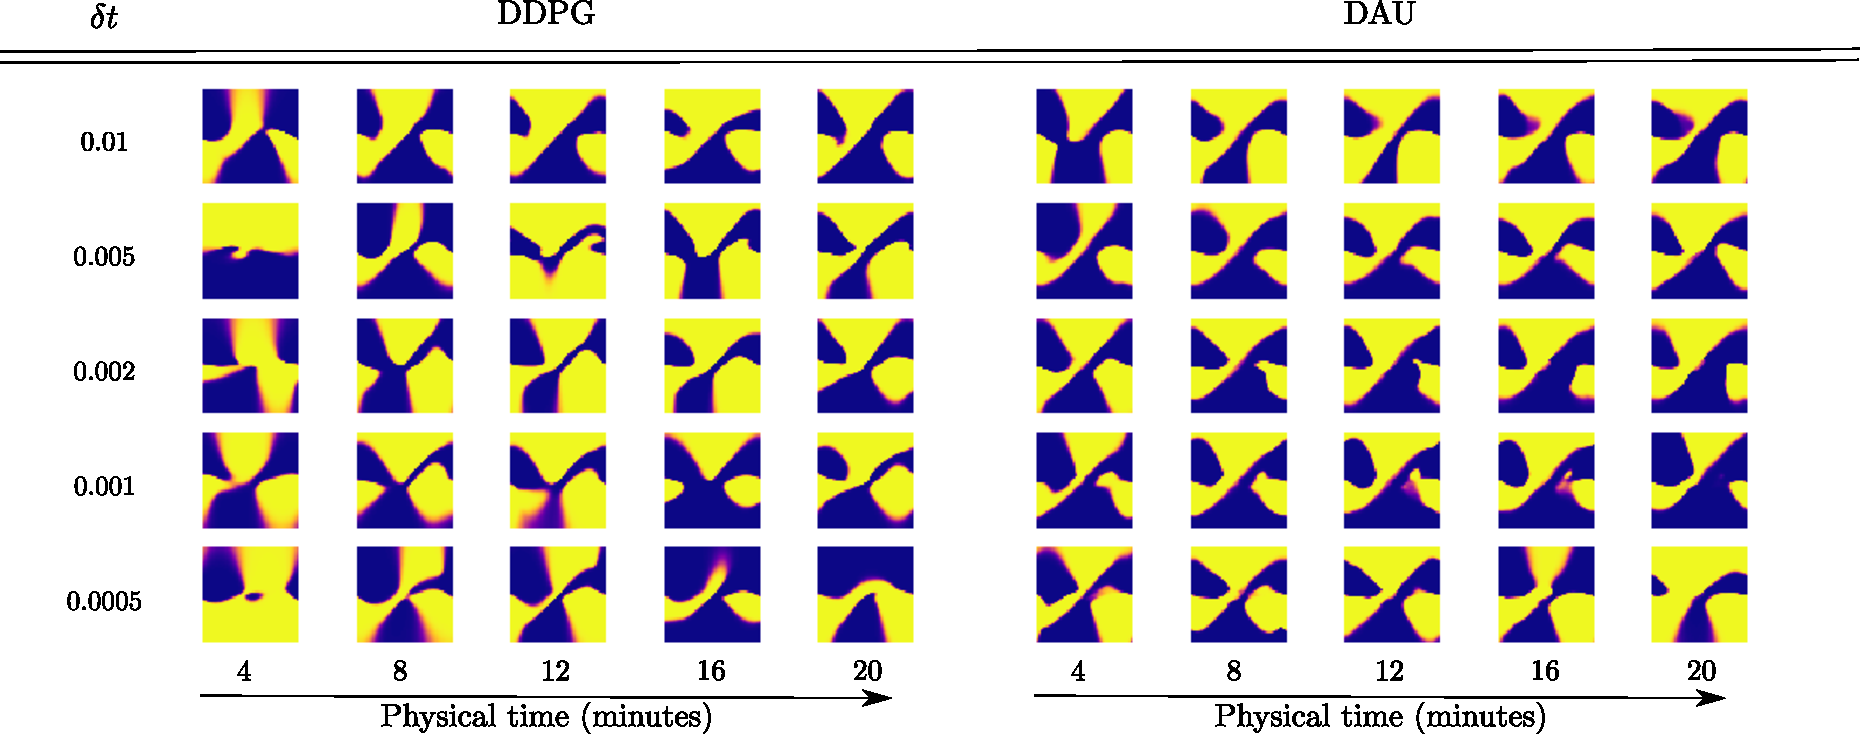
\includegraphics[width=\cw]{figs_data/pendulum_unscaled/pendulum_fig_act_unscaled.pdf}
	\caption{Policies obtained by DDPG (unscaled version) and AU at different instants in physical time of training on the pendulum swing-up environment. Each image represents the policy learnt by the policy network, with $x$-axis representing angle, and $y$-axis angular velocity. The lighter the pixel, the closer to $1$ the action, the darker, the closer to $-1$.}
        \label{fig:pend}
\end{figure*}
\begin{figure*}[h]
	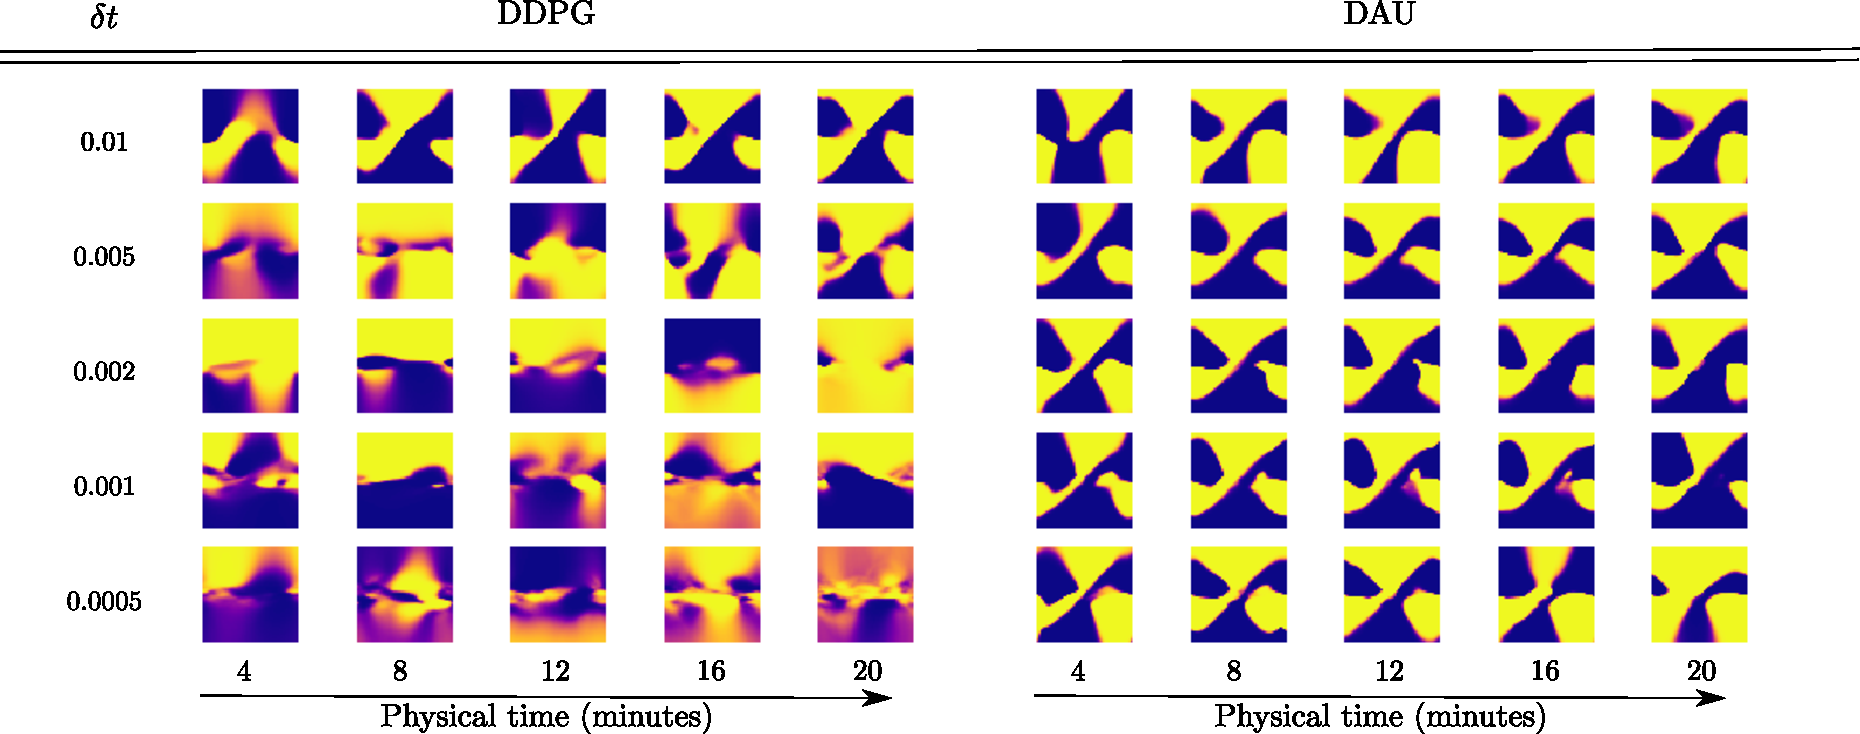
\includegraphics[width=\cw]{figs_data/pendulum_scaled/pendulum_fig_act_scaled.pdf}
	\caption{Policies obtained by DDPG (scaled version) and AU at different instants in physical time of training on the pendulum swing-up environment. Each image represents the policy learnt by the policy network, with $x$-axis representing angle, and $y$-axis angular velocity. The lighter the pixel, the closer to $1$ the action, the darker, the closer to $-1$.}
        \label{fig:pend}
\end{figure*}
\begin{figure*}[h]
	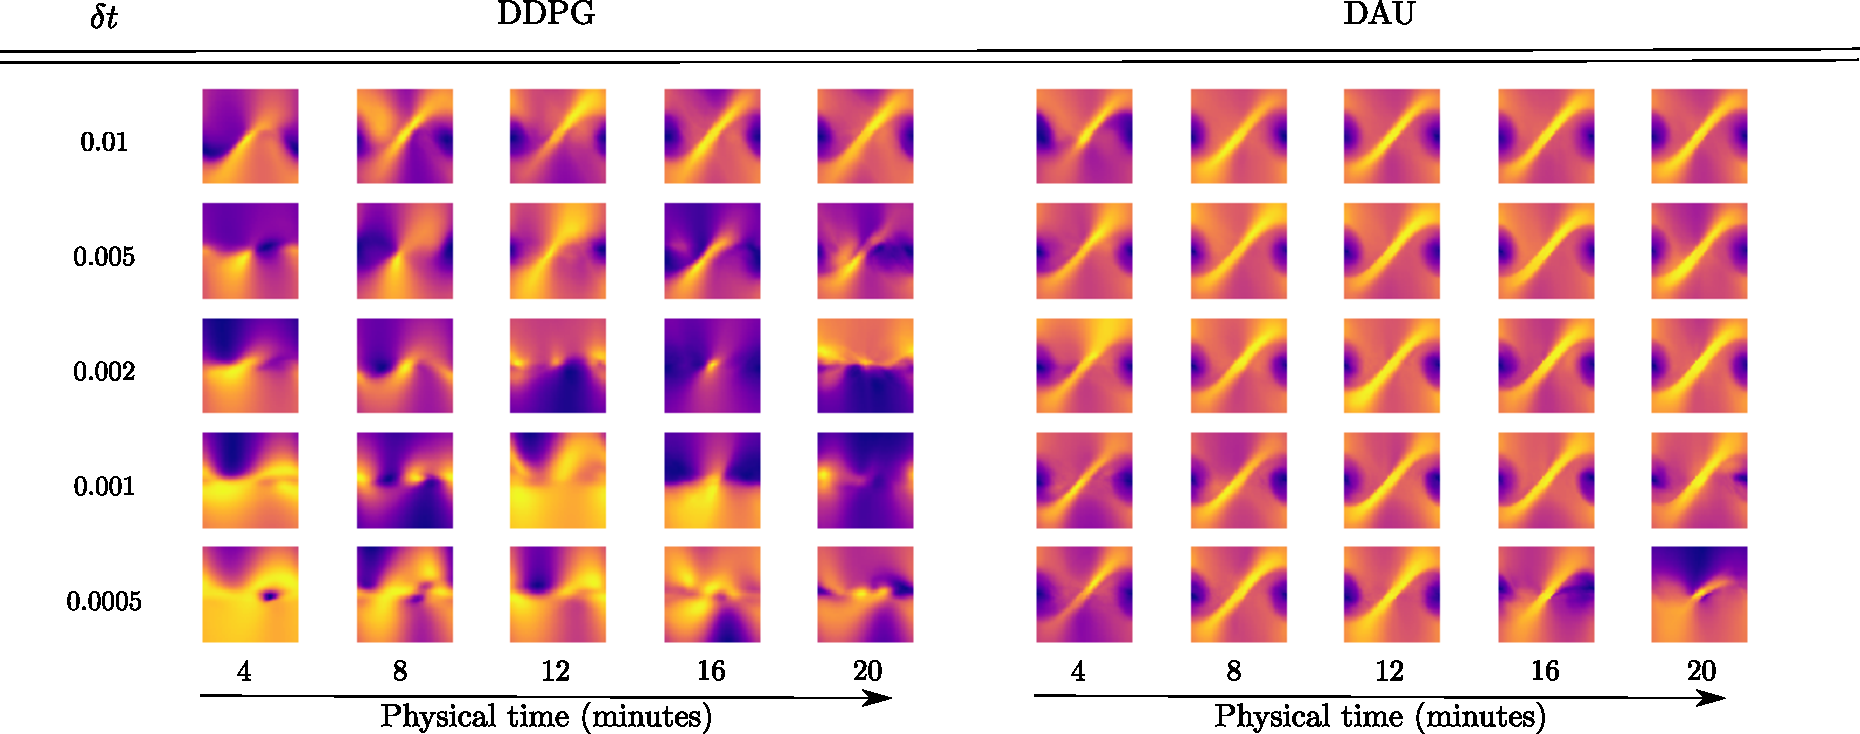
\includegraphics[width=\cw]{figs_data/pendulum_scaled/pendulum_fig_val_scaled.pdf}
	\caption{Value functions obtained by DDPG (scaled version) and AU at different instants in physical time of training on the pendulum swing-up environment. Each image represents the policy learnt by the policy network, with $x$-axis representing angle, and $y$-axis angular velocity. The lighter the pixel, the closer to $1$ the action, the darker, the closer to $-1$.}
        \label{fig:pend}
\end{figure*}

\end{document}
